\graphicspath{{./figures/}}

\section{Satellite Tracking}
There are various methods used to track satellites in order to keep maintain communication. Ultimately, all of these methods provide a single output to a ground station system: the direction in which to "steer" its antenna. Each method is compared and expanded on below.

\subsection{Open-Loop}
Arguably the simplest method is using what may be referred to as "open-loop" control. In this method, information about the flight path of the balloon is fed into the system, such as expected GPS co-ordinates at different points in time, and the ground station is simply pointed in that direction, with the "hopes" of maintaining a connection. The flight path can either be a pre-calculated path, or be continuously re-estimated based on realtime weather data. \textit{Habhub} is an online high-altitude path predictor \cite{site-stratoballooningPredictionTracking} which is freely available.

An advantage of this method is its extreme simplicity to implement. It has several disadvantages, however, including being vulnerable to prediction inaccuracies, as well as the difficulty experienced in re-acquiring the communication link once it is lost. Further, a GPS receiver is generally still required on the ground station, unless it is placed in a pre-determined location.

\subsection{GPS (Direct)}
If an initial communication link can be estabilished between the satellite and ground station, \textit{direct} GPS transmission can be added for positional feedback. This is a simple method of "closing" the tracking loop, since the path data can be updated dynamically.

Generally, both the PQ and GS GPS co-ordinates are required. Once these are retrieved, the GPS co-ordinates (known as the \textit{WGS84} system) can be \textit{projected} to a cartesian system using \textit{Mercator projection} \cite{site-mercator}.

\subsection{GPS (Relay)}
If a link cannot be initially estabilished, a "relay" method of GPS tracking can be used. This method functions in a three-step process, explained below and depicted in Figure \ref{fig:gps_relay}:
\begin{enumerate}
    \item The precise position of the payload and the ground station is determined using data received from GPS satellites.
    \item The position is \textit{relayed} to an external network (satellite or ground -based) using a radio transmitter.
    \item The ground station receives the location from the external network (e.g. via the internet).
\end{enumerate}

\begin{figure}[!htb]
  \centering
  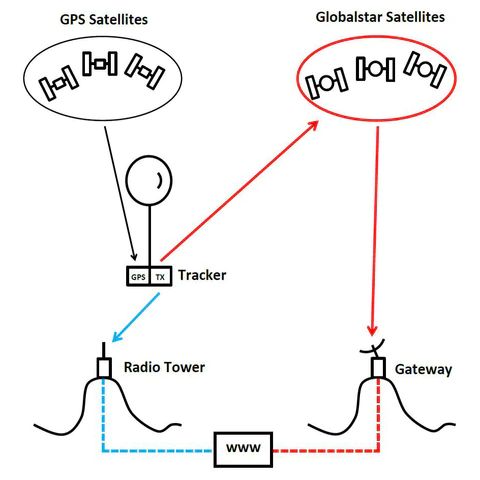
\includegraphics[width=0.3\textwidth]{gps_relay}
  \caption{GPS Relay Tracking \cite{site-highaltitudescienceTrackingWeather}}
  \label{fig:gps_relay}
\end{figure}

The major disadvantage of this method is the additional cost required. Since an antenna capable of communicating with one of the external networks is required, two antennas are needed if direct communication with a ground station is desired (however this is usually no longer necessary as the relay network can be used). Further, the cost of subscribing to an external network is generally high.

This type of tracking works well if the satellite is physically close to the external network satellites, or if the ground station does not need to communicate in realtime, but merely needs access to location of the satellite (e.g. in a homemade cellphone balloon satellite launch).

\subsection{Signal Strength}
Radio tracking can be done when the satellite itself transmits omni-directionally. The signal strength can then be used as feedback to determine the direction to point. To initially find the satellite, the entire sky can be scanned using a "brute force" procedure, or an initial guess can be provided. Then, periodic \textit{radius scanning} can be used to track the signal within a certain portion of the sky, or more advanced techniques such as \textit{conical scanning} can be used.